\chapter{Mapping} \label{chap:mapping}
    This chapter covers the mapping system used in this paper, starting with the process of projecting the depth image from the \ac{rgbd} camera into 3D space.
    After which, placing said 3D points into the heightmap buffer is covered. Finally the \ac{gpu} implementation of the heightmap processing is described.
    \section{Overview}
        For accurate foot placement and localisation purposes the robot makes use of two maps, a sparse map covering a large area, and a dense map covering a small
        area around the robot. The primarily use of the sparse map is for localisation and extracting pose data, i.e. orientation, velocity and rate. While the dense
        map is used to analyse the terrain and find an appropriate point to place the three supporting feet.
        It is possible to also use the sparse map for autonomous navigation, however this use case in not covered in this paper.
        This chapter covers the design of the mapping system.

        The localisation, sparse mapping and pose estimation is handle by ORB-SLAM3 as described in \cite{campos2021orb}. Since ORB-SLAM3 is not a system designed by the author, its
        design will not be covered in this chapter.

    \section{Projection}
        In order to generate a heightmap from a \ac{rgbd} image, it is first required to project the \ac{rgbd} image into 3D space, this is necessary because a heightmap is essentially a 3D environment,
        that can be represented as a image due to the assumption of purely convex geometry. 

        The camera can be described by its intrinsic and extrinsic parameters. Extrinsic parameters characterise the
        cameras position in 3D space, and intrinsic parameters characterise the relationship between the image plane and 3D space, 
        assuming the camera is at the world origin and an zero rotation \citep{hartley2003multiple}.

        Refer to figure \ref{fig:projection} as a visual aid regarding projection. Note that this figure is drawn from the perspective of projecting from the image plane into the world,
        if the objective was to project from the world onto the image plane the projection center and image plane would swap places, causing the image to be inverted, thus, this figure assumes
        that the image rotation has been corrected.
        \begin{figure}[h]
            \centering
            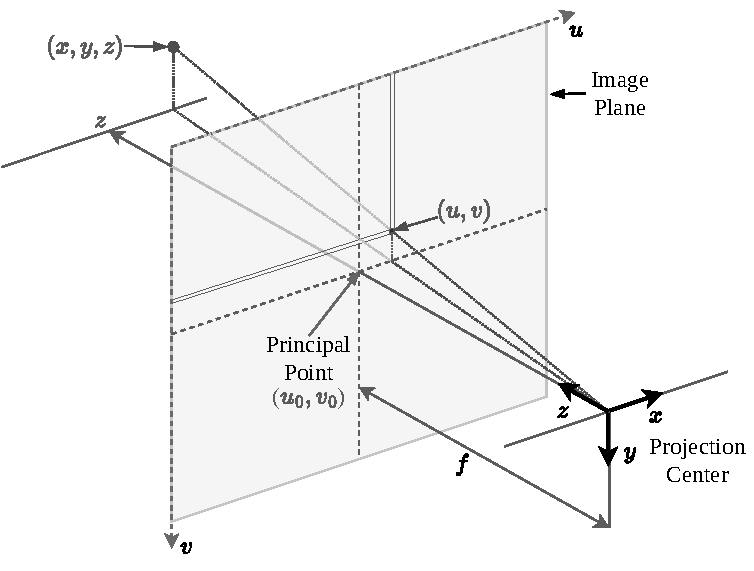
\includegraphics{Diagrams-Projection.drawio.pdf}
            \caption{Camera Projection}
            \label{fig:projection}
        \end{figure}

        \noindent
        Together the extrinsic and intrinsic matrices form the projection matrix,
        as shown in equation \ref{eq:projection_matrix},
        \begin{equation} \label{eq:projection_matrix}
            \bm{P} = \bm{K}
            \begin{bmatrix}
                \bm{R} & \bm{T}
            \end{bmatrix}
        \end{equation}
        where \(\bm{K}\) is the intrinsic matrix and \(\begin{bmatrix} \bm{R} & \bm{T} \end{bmatrix}\) the extrinsic matrix, these are described
        in equation \ref{eq:intrinsic} and \ref{eq:extrinsic}.
        The projection matrix can be used to project a point on the image plane into world space as shown in equation \ref{eq:full_projection}.

        \begin{equation} \label{eq:full_projection}
            \begin{bmatrix}
                u \\
                v \\
                1
            \end{bmatrix}
            = \bm{P}
            \begin{bmatrix}
                x \\
                y \\
                z \\
                1
            \end{bmatrix}
        \end{equation}
        where \(u,v\) are the pixel coordinates on the image plane and \(x,y,z\) are the coordinates in world space.

        The intrinsic matrix \(\bf{K}\) is defined as such,
        \begin{equation} \label{eq:intrinsic}
            \bm{K} =
            \begin{bmatrix}
                \alpha_x & \gamma   & u_0 \\
                0        & \alpha_y & v_0 \\
                0        & 0        & 1
            \end{bmatrix}
        \end{equation}
        where the focal length is represented by,
        \[\alpha_x = f \cdot m_y\]
        \[\alpha_y = f \cdot m_x\]
        with \(m_x\) and \(m_y\) being the inverse of the width and height of a image plane pixel, \(f\) the focal length and \(u_0\),\(v_0\) being the principal point, optimally the center of the image plane.
        The skew coefficient, \(\gamma\), is often, and in this case, 0.

        The extrinsic matrix is as shown below,
        \begin{equation}\label{eq:extrinsic}
            \begin{bmatrix}
                \bm{R} & \bm{T}
            \end{bmatrix}
            =
            \begin{bmatrix}
                \bm{R}_{3\times3} & \bm{T}_{3\times1} \\
                \bm{0}_{1\times3} & 1
            \end{bmatrix}
        \end{equation}
        where \(\bm{R}\) characterises the camera's heading in world space and \(\bm{T}\) the world origin expressed in 
        the camera coordinate frame.

        For ease of preprocessing points are first projected into the camera coordinate frame, in other words, the extrinsic matrix is omitted from equation \ref{eq:full_projection}.
        The resultant matrix equation is shown in equation \ref{eq:local_projection}.

        \begin{equation} \label{eq:local_projection}
            \begin{bmatrix}
                u \\
                v \\
                1 \\
                1/z
            \end{bmatrix}
            = \frac{1}{z}
            \begin{bmatrix}
                f_x & 0 & c_x & 0 \\
                0 & f_y & c_y & 0 \\
                0 & 0 & 1 & 0 \\
                0 & 0 & 0 & 1
            \end{bmatrix}
            \begin{bmatrix}
                x\\
                y\\
                z\\
                1
            \end{bmatrix}
        \end{equation}
        From equation \ref{eq:local_projection} \(x,y,z\) are found to be show in equation \ref{eq:proj_z} to \ref{eq:proj_y}.
        \begin{align}
            z &= I_{u,v} \label{eq:proj_z}\\[0.2cm]
            x &= \frac{z(u - u_0)}{\alpha_x}\label{eq:proj_x} \\
            y &= \frac{z(v - v_0)}{\alpha_y}\label{eq:proj_y}
        \end{align}
        where \(I_{u,v}\) is the depth image value at pixel coordinates \(u,v\). For later use the variable \(\bm{p} \inrefframe{C}\) is defined as in equation \ref{eq:pcam},
        \begin{equation}\label{eq:pcam}
            \bm{p}\inrefframe{C}=
            \begin{bmatrix}
                x &y &z
            \end{bmatrix}^T
        \end{equation}

    \section{Map Buffer}
        Once the depth image is projected into map space, their x and y coordinates are used as indices to write their z value into the heightmap. The heightmap is stored in
        a 2D circular buffer, this means that as the robot moves around, old map data is erased to make room for new data. This structure is illustrated in figure \ref{fig:memory}.
        \begin{figure}[h]
            \centering
            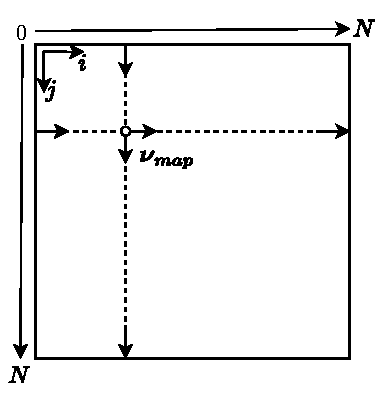
\includegraphics{Diagrams-Memory.drawio.pdf}
            \caption{Memory Diagram}
            \label{fig:memory}
        \end{figure}

        \noindent
        The heightmap buffer, \(\bm{M}\), is of size \(N \times N\) and is indexed by \(i,j\). In order to write the height value into the heightmap, the camera point in camera space,
        \(\bm{p}\inrefframe{\fcamera}\), is translated into map space, \(\bm{p}\inrefframe{\fmap}\), as shown in equation \ref{eq:project_to_map},
        \begin{equation} \label{eq:project_to_map}
            \bm{p}\inrefframe{\fmap} = \transframe{\bm{p}\inrefframe{\fcamera}}{\fcamera}{\fmap}
        \end{equation}
        where \transframe{\bm{x}\inrefframe{\fcamera}}{\fcamera}{\fmap} is defined as in equation \ref{eq:camera_to_map},
        see appendix \ref{app:transforms} for more information.
        \begin{align} \label{eq:camera_to_map}
            \begin{split}
                \bm{x}\inrefframe{\fmap} &= \transframe{\bm{x}\inrefframe{\fcamera}}{\fcamera}{\fmap}\\ 
                &= (\bm{q}_\text{cam} \cdot \bm{x}\inrefframe{\fcamera} \cdot \bm{q}_\text{cam}^{-1}S + \bm{p_\text{rob}}\inrefframe{\fmap}) \mod N
            \end{split}
        \end{align}

    \newpage
    \section{GPU Compute Pipeline}
        As the heightmap generation and heightmap scoring systems are essentially image manipulation processes, parallelisation of the algorithms
        is a very efficient way to increase computational speeds, thus, these algorithms are run in parallel on the Jetson nano's \ac{gpu} using OpenGL
        compute shaders. This section describes the compute pipeline used to build and score the heightmap. The compute pipeline can be seen in
        figure \ref{fig:compute_pipe}.
        \captionsetup[figure]{oneside,margin={0cm,0cm}}
        \begin{figure}[h]
            \centering
            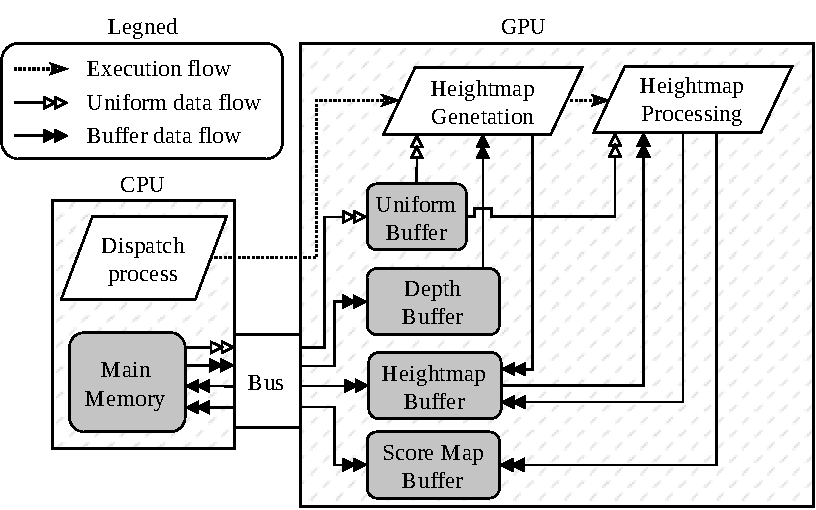
\includegraphics{Diagrams-ComputePipeline.drawio.pdf}
            \caption{Compute pipeline.}
            \label{fig:compute_pipe}
        \end{figure}
    
        \noindent
        As seen from figure \ref{fig:compute_pipe} the \ac{gpu} pipeline is relatively simple, being comprised of only two stages, the heightmap generation
        stage and the heightmap processing stage. The heightmap generation stage executes for each pixel on the depth image, constructing the heightmap as 
        described in chapter \ref{chap:mapping}.
        
        After the heightmap has been generated, the heightmap processing stage operates over the heightmap buffer. This stage has two tasks, to erase the
        old height data as the robot walks around, and to generate the score map, as described in section \ref{sec:scores}.
        
        \newpage
        \subsection{A note on \ac{gpu} architecture}
            A process on a \ac{gpu} operates fully in parallel and the \ac{gpu} is highly optimised for parallelisation, thus there is a very specific
            execution structure that a \ac{gpu} process abide by to perform at maximum efficiency, or to even function at all. This execution structure is
            as follows.
            
            As per \cite{nvidia_doc}, when writing compute code a 3D size is specified, the localgroup size, \(\bm{N}_{l} = [X_l,Y_{l},Z_{l}]\), next when the \ac{cpu} dispatches
            a compute task, the workgroup count, is fed as parameter, \(\bm{n}_{w} = [x_{w},y_{w},z_{w}]\). The \ac{gpu} then initialises
            \(\bm{n}_w\) workgroups, and each workgroup initialises \(\bm{N}_l\) threads. These threads are executed into warps, or waves, which, depending on the architectures processor count,
            can be either 32 or 64 threads. To ensure maximum efficiency it is important that \(\bm{N}_l\) is divisible by the warp size.
            Originally Nvidia \ac{gpu}s utilised a warp size of 32 and AMD 64, however with AMDs latest RDNA architecture, the warp size could be either 32 or 64.
            This system assumes a warp size of 32.
            
            For the heightmap generation stage \(\bm{N}_{l} = [32,32,0]\) for a total of 1024 threads per workgroup, or in other words, 32 warps per workgroup.
            As for the heightmap processing stage, \(\bm{N}_{l} = [32,32,32]\), meaning 32768 threads, or 1024 warps per workgroup.
            As such it is important that camera images, the heightmap and the score map are of a size divisible by 32.
            % A basic diagram of this execution scheme can be seen in figure \ref{fig:gpu_scheme}.
            % \begin{figure}[h]
            %     \centering
            %     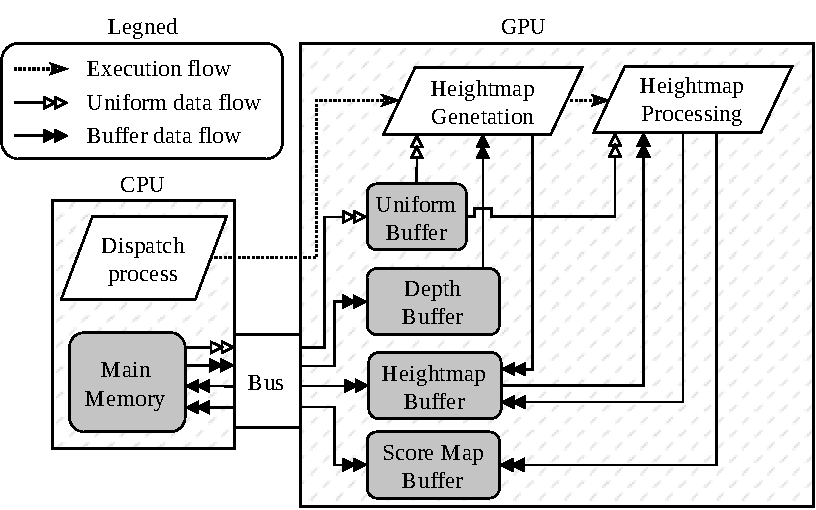
\includegraphics{Diagrams-ComputePipeline.drawio.pdf}
            %     \caption{GPU execution scheme.}
            %     \label{fig:gpu_scheme}
            % \end{figure}
        
            % \noindent
            While threads can directly communicate with each other within the same workgroup, direct communication across workgroups is
            impossible. If cross workgroup communication is desired, this must be performed using \ac{gpu} buffers, which are slower to access. Thus processes are
            designed to operate fully independently from each other. Of course, data transfer between the \ac{cpu} and the \ac{gpu} is orders of magnitudes
            slower than accessing local buffers, as such, all \ac{cpu}, \ac{gpu} communication is kept to a minimum.
            
            Finally it should be noted that while it is possible to vary \(\bm{s_w}\) with each execution cycle, \(\bm{S_l}\) is a constant specified at compile time,
            and as such the number of threads per workgroup cannot be altered during operation.

    \newpage
    \section{Hardware Mapping Test}\label{sec:hardware_hmap}
        The mapping system described above was tested on the physical robot, this mapping test aims to show how the physical hexapod maps various objects while in motion.
        The test consists of the robot walking past various obstacles, while simultaneously generating a heightmap.

        Figure \ref{fig:hardware_map_diag} shows a top-down diagram of the placed obstacles used in this test, with the path the robot walks.
        \begin{figure}[h]
            \centering
            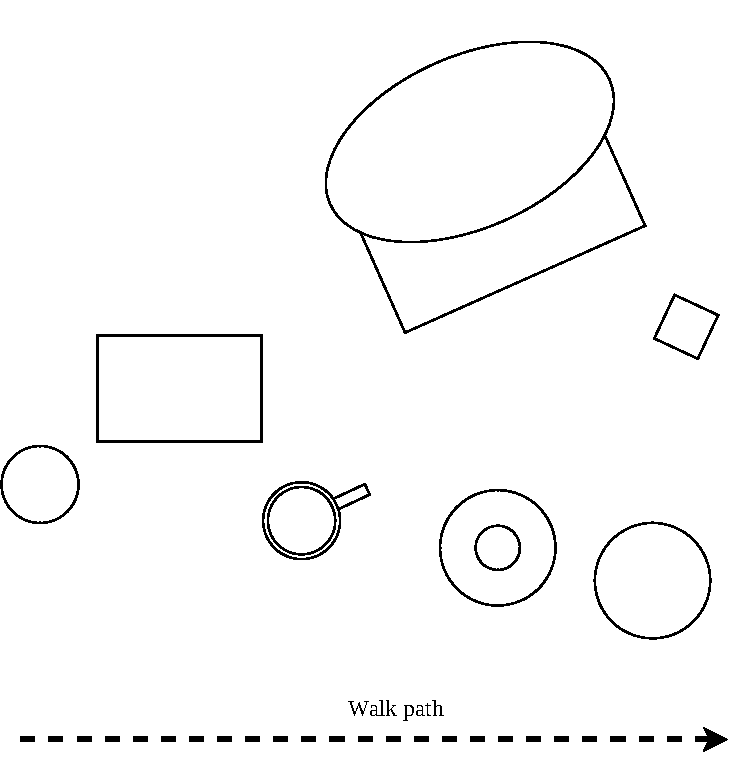
\includegraphics{Diagrams-HardwareTest.drawio.pdf}
            \caption{Top-down diagram of the test setup.}
            \label{fig:hardware_map_diag}
        \end{figure}

        \noindent
        The test objects were selected to show a variety of obstacle types, with a variety of heights, that the robot might encounter, including sloped objects, spherical objects, objects
        with holes and irregular objects. 

        Figures \ref{fig:hardware_hmap_start}, \ref{fig:hardware_hmap_mid} and \ref{fig:hardware_hmap} show the heightmap, and its corresponding color frame, at the start middle and end of the
        robot's walking path.
        
        \newpage
        \noindent
        Figure \ref{fig:hardware_hmap_start} shows the heightmap at the start of the generation, at this point the heightmap is essentially a direct representation of what is
        currently seen by the camera. This is uie clear by the shadows cast by both the robot's leg (on the left) and by the obstacles (the pig and box). In this static case
        very little noise is also present.
        \begin{figure}[h]
            \centering
            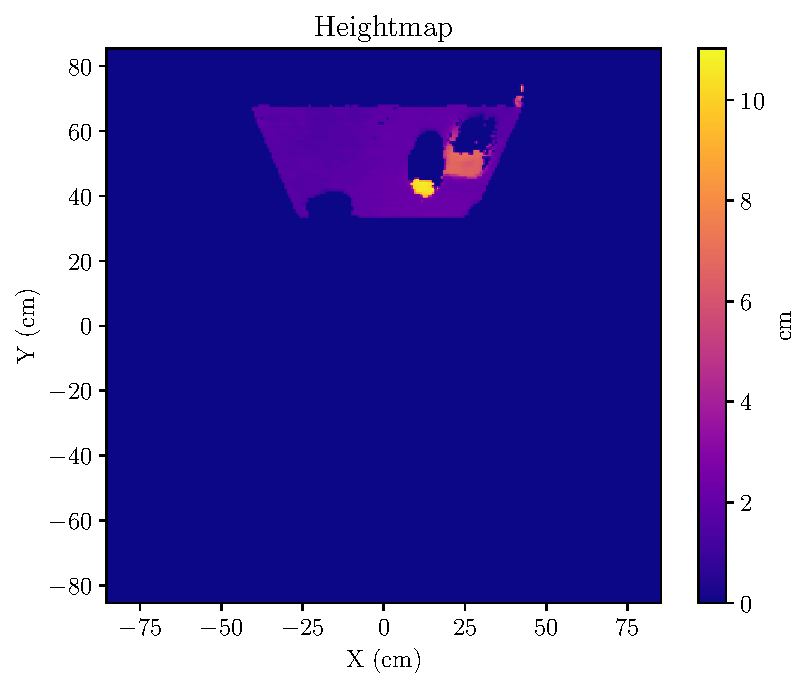
\includegraphics{hmap_start.pdf}
            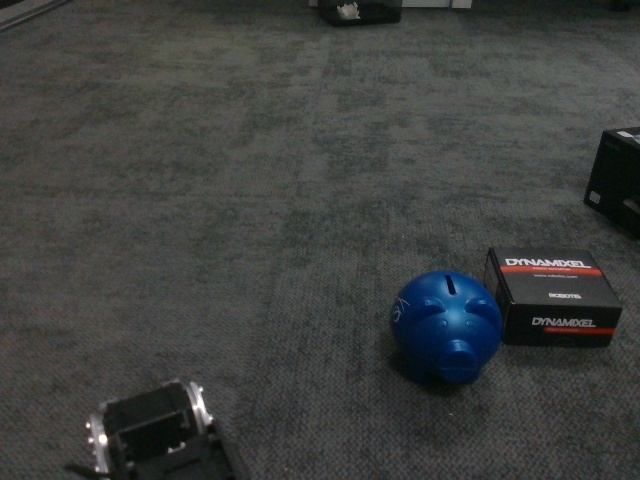
\includegraphics[width=.5\textwidth]{color_start.jpeg}
            \caption{Heightmap generated at the start of the walking path (Top). Color frame at the start of walking path (Bottom).}
            \label{fig:hardware_hmap_start}
        \end{figure}
        
        \newpage
        \noindent
        Figure \ref{fig:hardware_hmap_mid} shows the heightmap at a middle point of the path, here it can be seen how some of the shadows have been
        filled in by the movement of the camera. Particularly, the shadow caused by the robot leg is no longer present, and the shadows cast by the
        obstacles are reduced. The somewhat spherical pig object now also appears larger as part of the other side became visible.
        \begin{figure}[h]
            \centering
            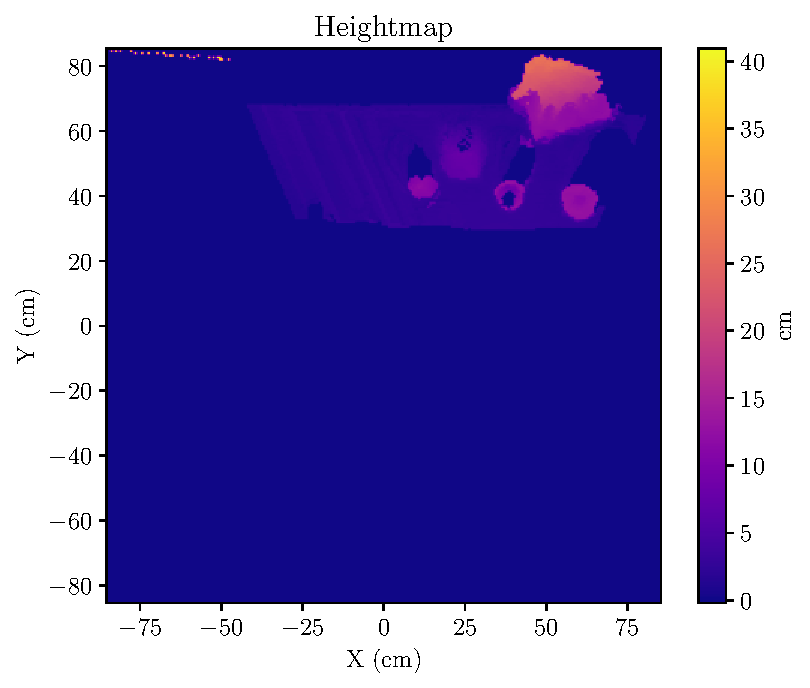
\includegraphics{hmap_half.pdf}
            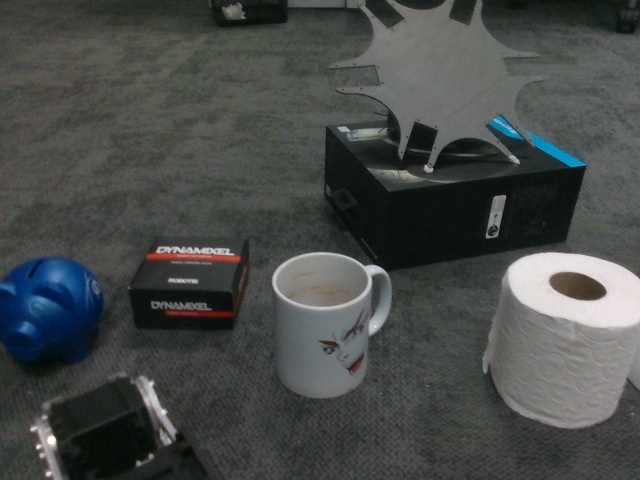
\includegraphics[width=.5\textwidth]{color_half.jpeg}
            \caption{Heightmap generated at the middle of the walking path (Top). Color frame at the middle of walking path (Bottom).}
            \label{fig:hardware_hmap_mid}
        \end{figure}

        \noindent
        In this heightmap however, noise is more prevalent, this is particularly visible when looking at the floor height, where distinct lines can be observed.
        These lines are the edge of the field of vision of the camera which is being moved to the right, and is caused by inaccuracies in the position estimation.

        \begin{figure}[h]
            \centering
            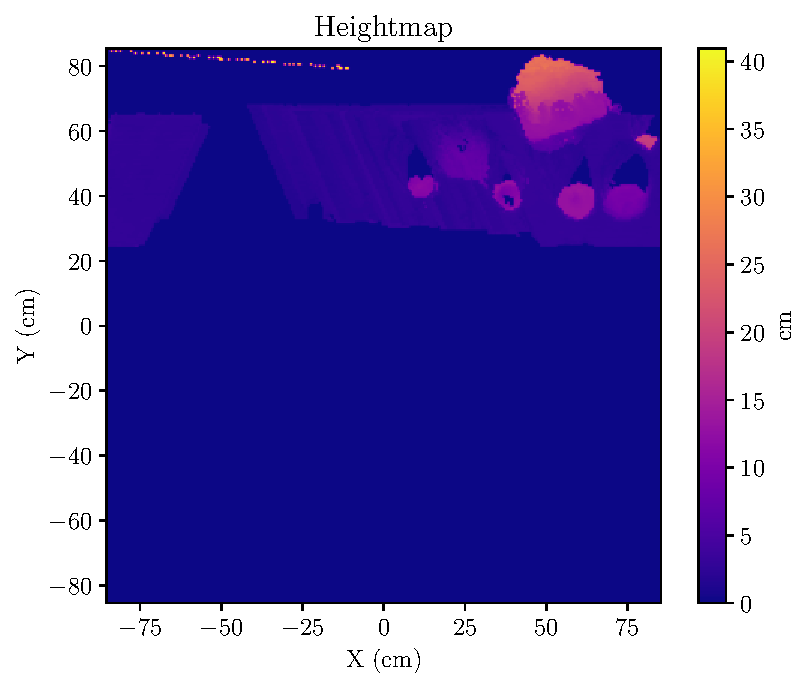
\includegraphics{hmap.pdf}
            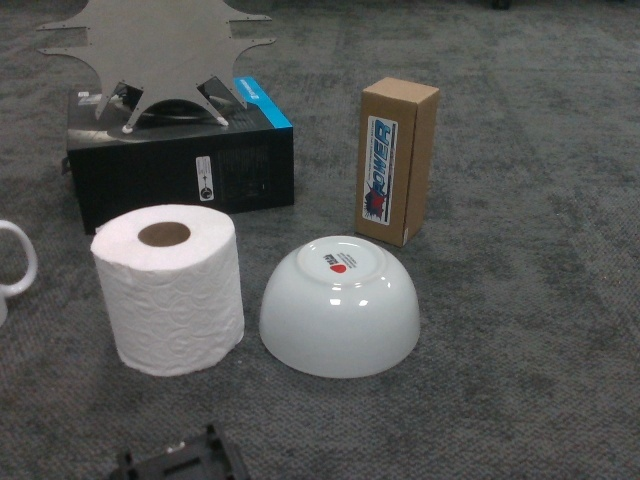
\includegraphics[width=.5\textwidth]{color.jpeg}
            \caption{Heightmap generated at the end of the walking path (Top). Color frame at the end of walking path (Bottom).}
            \label{fig:hardware_hmap}
        \end{figure}

        \noindent
        Finally, the heightmap generated at the end of the walking path can be seen in figure \ref{fig:hardware_hmap}. In this heightmap the shadows cast
        have been shrunk even more, and some additional objects became visible. The original objects are also now out of vision, but they persist on the heightmap. 

        Figure \ref{fig:hardware_pos} shows the robot's estimated position, with each dot being a estimation. The blue dot is the start of the test and the red dot the end of the test.
        \begin{figure}[h]
            \centering
            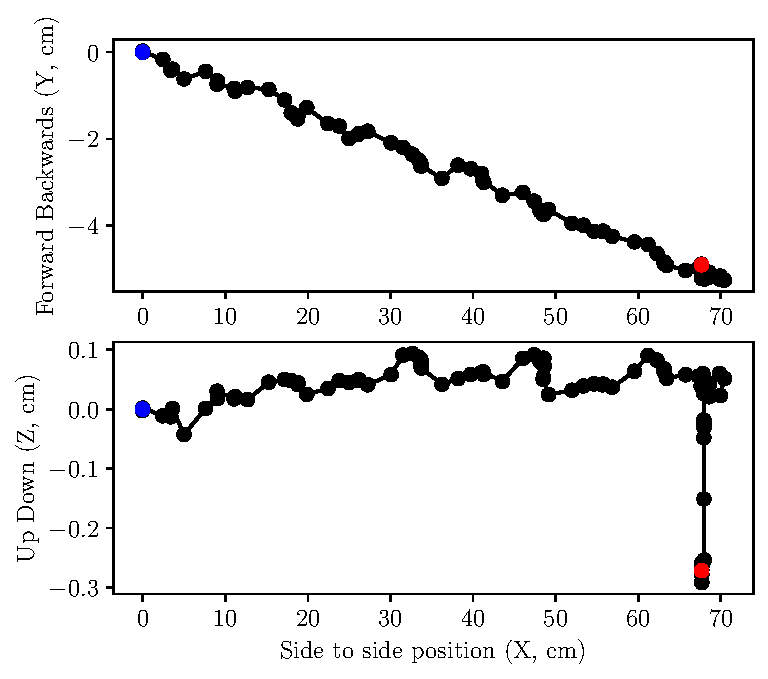
\includegraphics{pos.pdf}
            \caption{Position output from ORB-SLAM3}
            \label{fig:hardware_pos}
        \end{figure}

        \noindent
        As can be seen, the frequency of pose estimation causes there to sometimes be large jumps between estimations. This is especially noticeable at the end where the
        robot quickly lowers itself. If the system was further optimised to increase the frequency and consistency of estimations the accuracy of the heightmap
        would also increase.

        Note that the line of motion is not aligned perfectly with the x-axis as stated in the test diagram in figure \ref{fig:hardware_map_diag}, this is due to slight user
        error while inputting the target velocity, but does not have any negative effects on the resultant heightmap.
    % \bigskip
    % \bigskip
    % \hrule
    % \smallbreak
    % \hrule
